\documentclass[epsfig,11pt]{article}
\usepackage[english]{babel} % Using babel for hyphenation
\usepackage{lmodern} % Changing the font
\usepackage[utf8]{inputenc}
\usepackage[T1]{fontenc}

\usepackage{amssymb}
\usepackage{graphicx}
\usepackage{amsmath}
\usepackage{epsfig}
\usepackage[parfill]{parskip} % Removes indents

\usepackage{vmargin}
\setpapersize{A4}

\newcommand{\inr}[1]{ \Big \langle #1 \Big \rangle}
\newcommand\pd[2][]{\ensuremath{\frac{\partial#1}{\partial#2}}} 

\title{Applications of finite element methods in biomechanics}
\author{Krister Stræte Karlsen}

\begin{document}

\maketitle

\section{Stokes flow in zebrafish}

Since the 1960s, the zebrafish has become increasingly important to scientific research. It has many characteristics that make it a valuable model for studying human genetics and disease. It was the first vertebrate to be cloned and is particularly notable for its regenerative abilities. Zebrafish have a similar genetic structure to humans. They share 70 per cent of genes with us and they are cheaper to maintain than mice. The zebrafish adult is about 2.5 cm to 4 cm long. 

To study the effect of different drugs being able to model the blood flow is important. For instance, if the drug actually never reaches the infected cells a potentially effective drug might be considered ineffective on wrong the wrong basis. 

The blood velocities in a zebrafish are low thus using \emph{Stokes flow} as a model is a fair approximation.

 \begin{figure}[h!] 
\begin{center}
  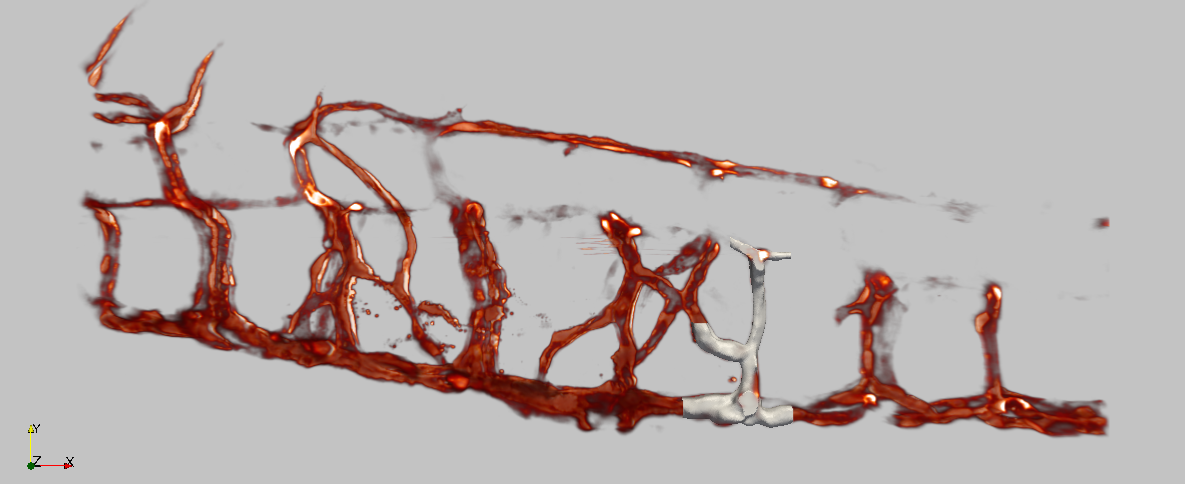
\includegraphics[scale=0.3]{overview2.png}
  \end{center}
  \caption{The circulatory system of a zebrafish where a small part is meshed.}
\end{figure}

\begin{figure}[h!] 
\begin{center}
  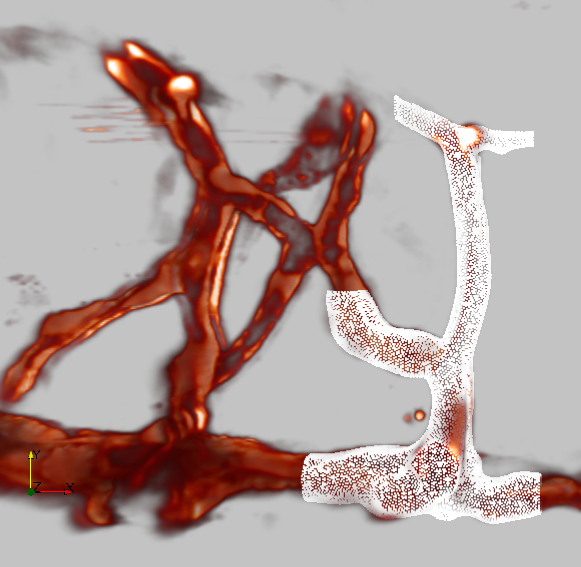
\includegraphics[scale=0.3]{zoomed2.png}
  \end{center}
  \caption{Zooming in to see the meshed region.}
\end{figure}

\subsection{Mathematical formulation}


\section{Squeezing a postdoc's brain}

We would very much like to squeeze postdoc Erika Lindström's brain. Since she has refused to let us do this with our hands in her office, we must do this on a computer using her brain as our computational domain. The brain will be deformed as a result of the squeezing and to capture this effect we will use a \emph{linear elastic} model. 

A mesh of Erika's brain can be found in the git repository:
 https://github.com/krikarls/fun-with-fem. 
 
 \begin{figure}[h!] 
\begin{center}
  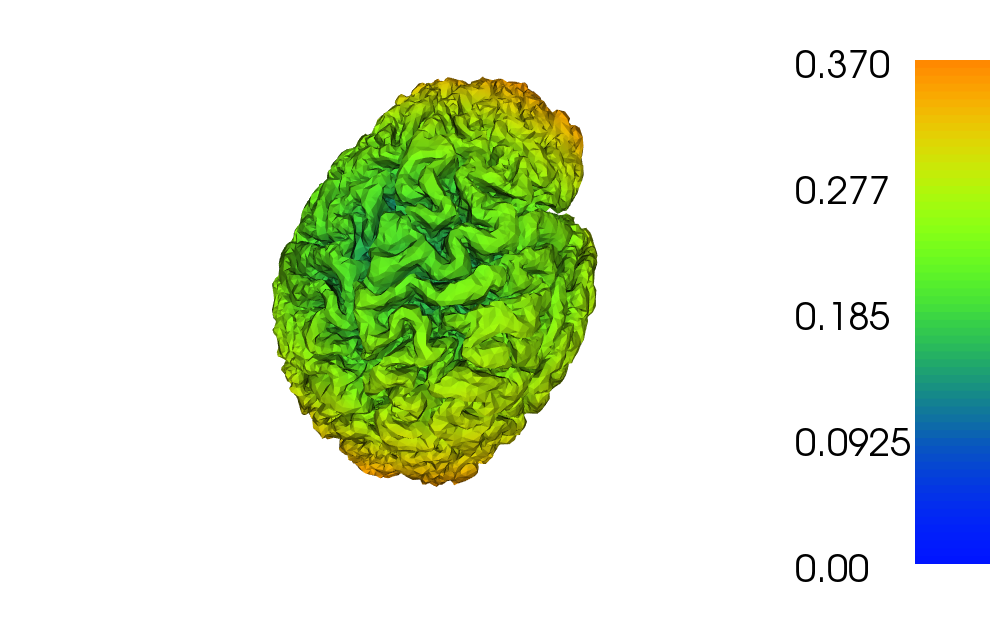
\includegraphics[scale=0.4]{brain.png}
  \end{center}
  \caption{Numerical solution using FEniCS. Displacement measured in $mm$.}
\end{figure}

The brain is not clamped in the skull, but in a sence floating around. This means that we must employ \emph{neumann booundary conditions} on the entire boundary. As we know, there are no unique solution to such a problem since all \emph{rigid motions} satify the equation. So in order to obtain a unique solution we must remove all rigid motions. All the possible rigid motions in 3D are: translations in $x,y,z$-direction and rotations around the corresponding axes. Thus six in total.

An example using \emph{FEniCS} on how to remove these can be found in the same repository as the brain. 

\subsection{Mathematical formulation}

\end{document}
